\section{Authentication}

\subsection{Configuration}

Configuring an Auth0 provider starts with an
\enquote{application}, which represents the system it's
serving (i.e., the frontend).
Once the application type is set to SPA, the token signing
algorithm is limited exclusively to RS256 since an
\gls{SPA} cannot store secrets in the browser, instead
requiring a public \& private key-pair for asymmetric
encryption. As per the design, all authentication
mechanisms aside from socials were disabled.

In the frontend, the authentication flow utilises the SDK
offered by Auth0 for Vue 3, requiring the provider's
domain, client\_id, and audience which is stored in
environment files:

\lstinputlisting{06 implementation/assets/auth0 sdk.ts}

Navigation guards in Vue Router also leverage the SDK using
the \lstinline{isAuthenticated} flag before directing to
authenticated pages.

From here, the designs from the \enquote{Authentication}
\hyperref[ss:stories]{user story} were implemented to
produce an authentication flow shown in Figure
\ref{fig:authFlow}.

\begin{figure}
  \centering

  \begin{subfigure}{\subfigwidth}
    \centering
    \frame{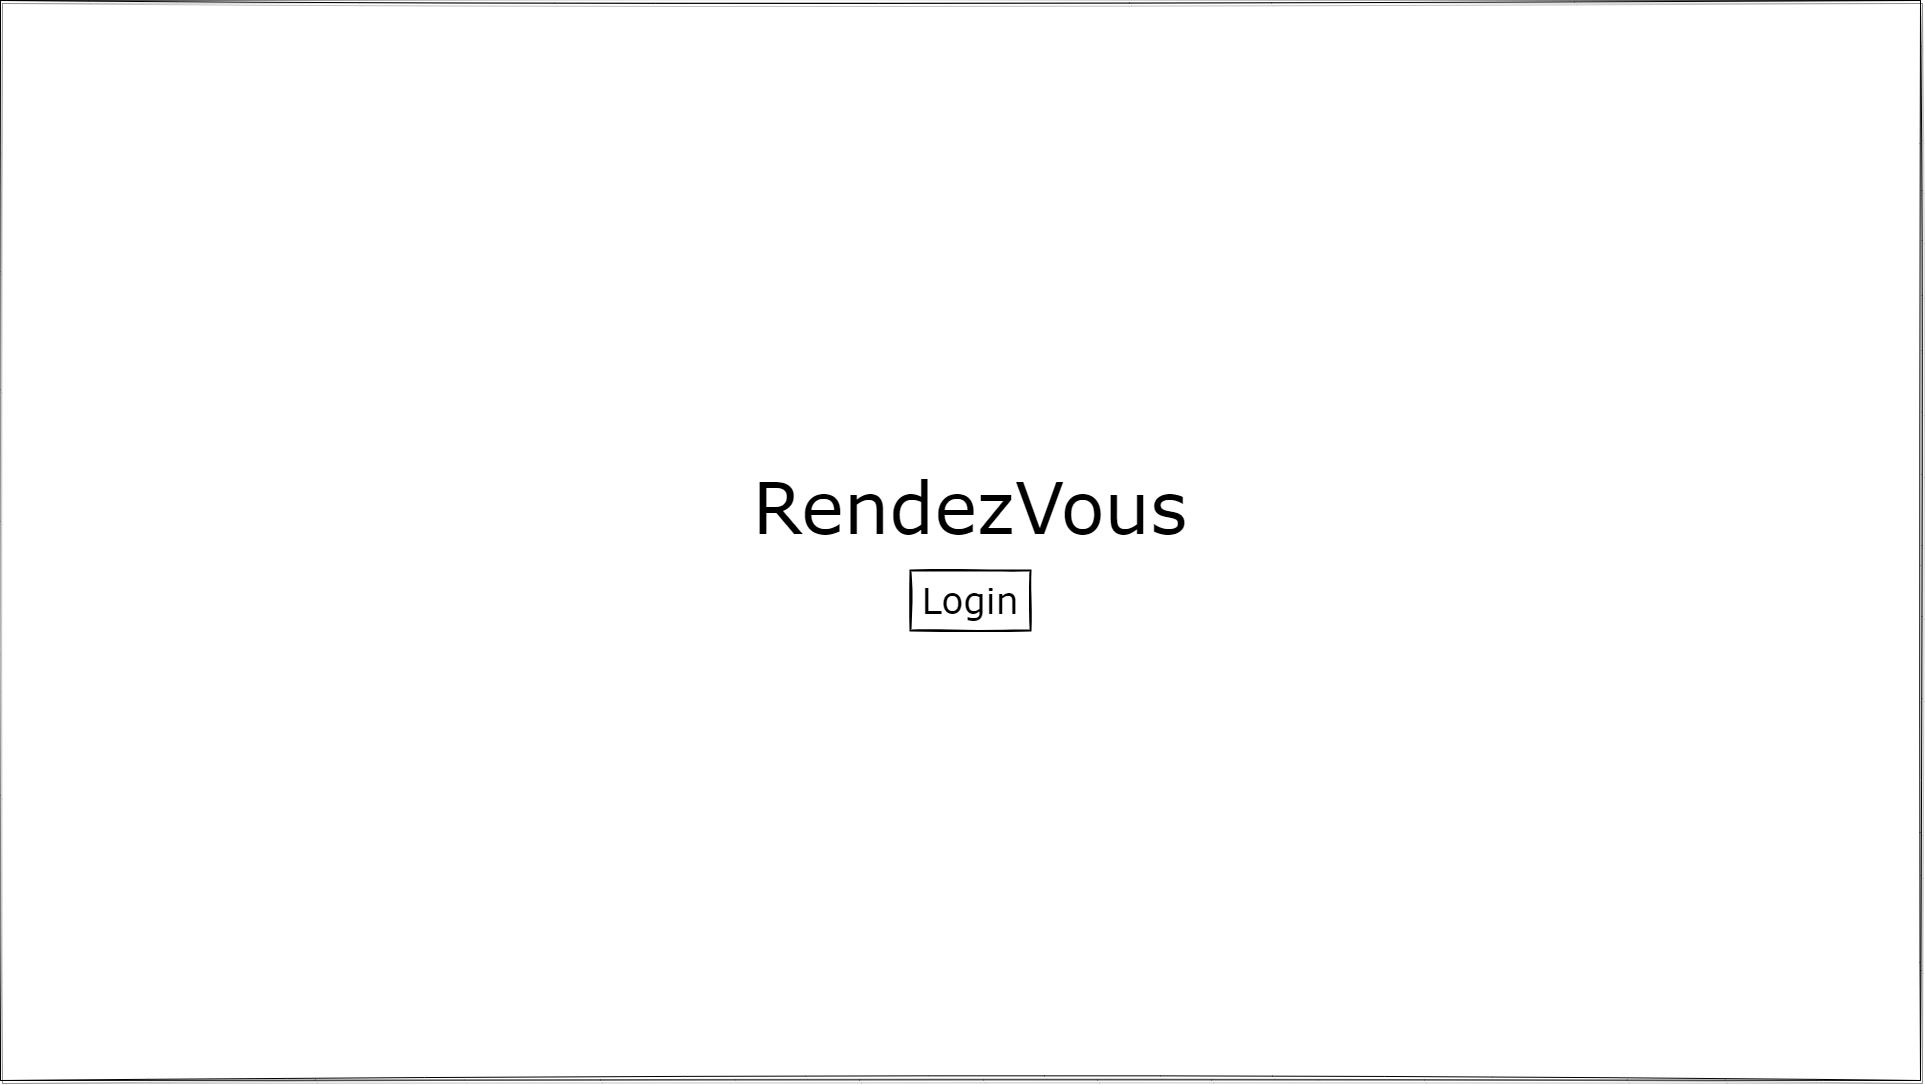
\includegraphics[width=0.9\linewidth]{06
        implementation/assets/auth flow/home page no auth.png}}
    \caption{Home page before authenticating}
  \end{subfigure}
  \begin{subfigure}{\subfigwidth}
    \centering
    \frame{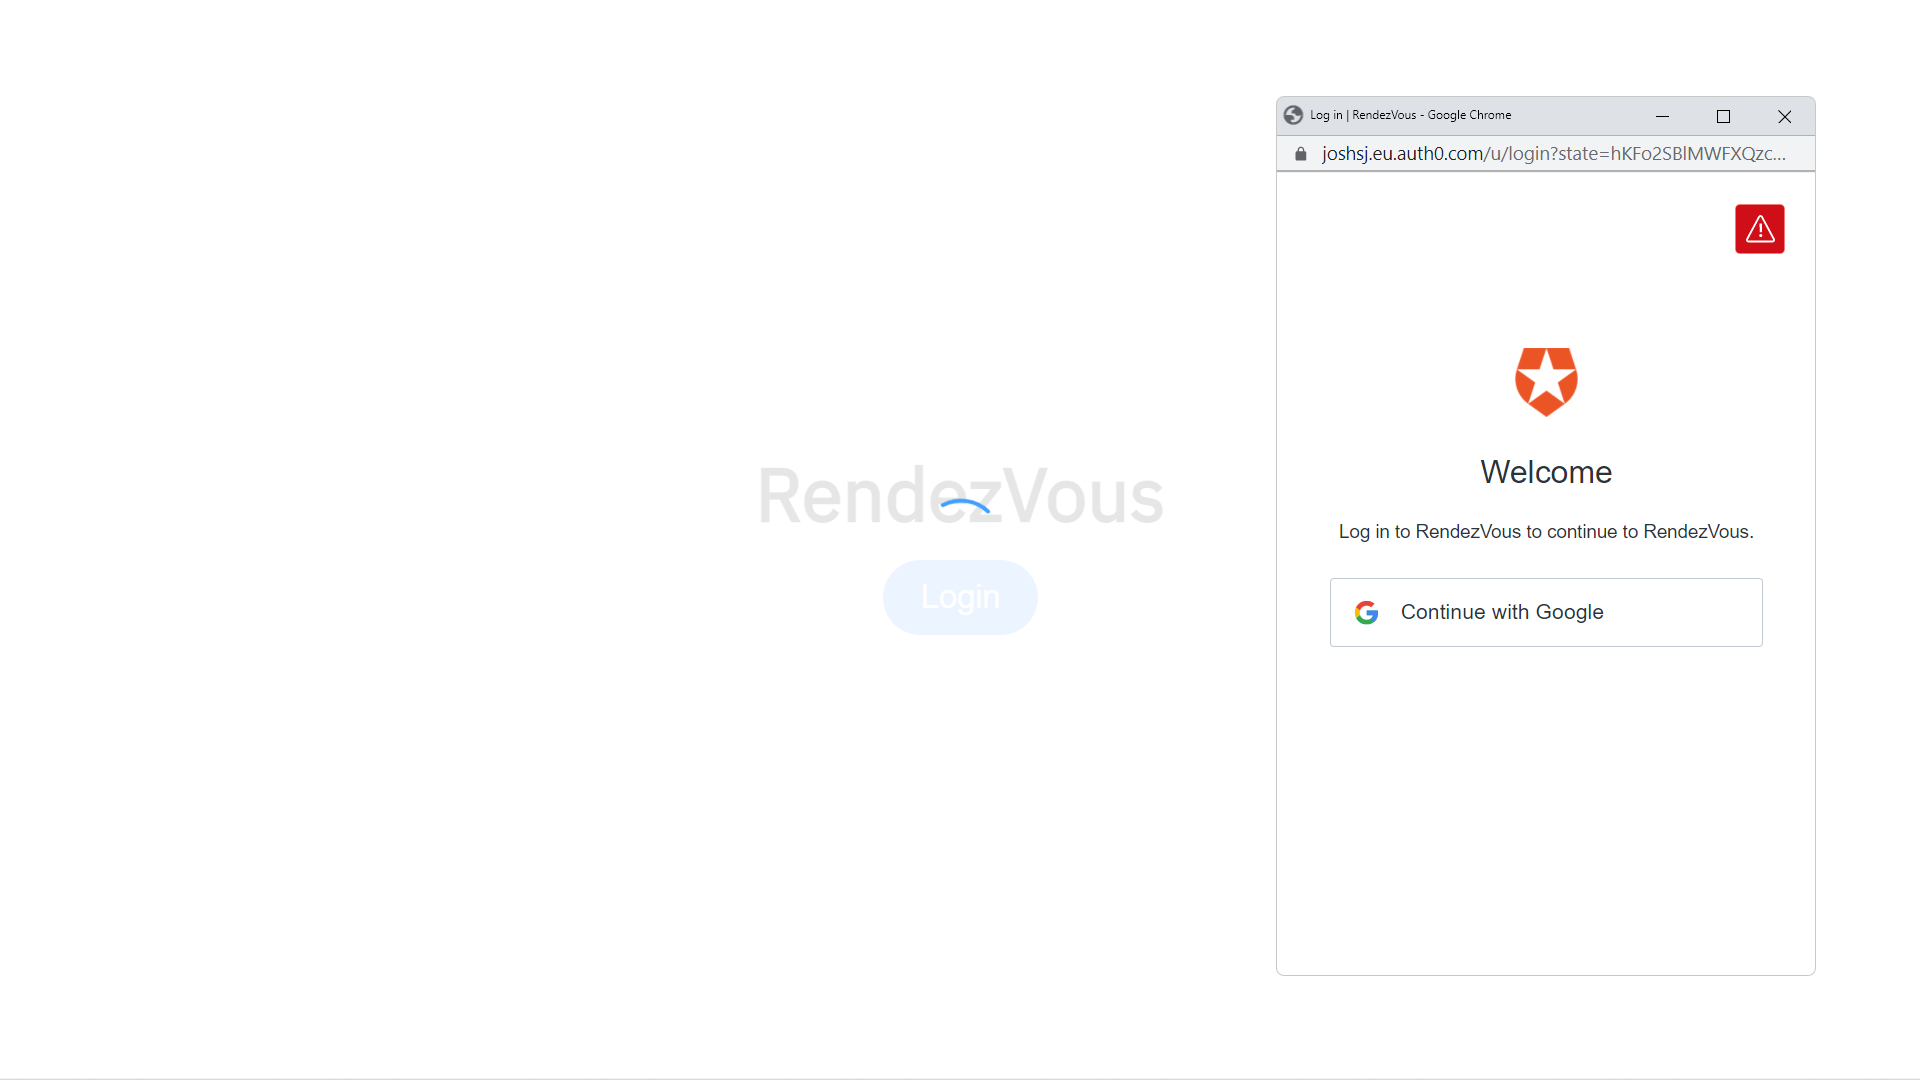
\includegraphics[width=0.9\linewidth]{06
        implementation/assets/auth flow/auth popup.png}}
    \caption{Authentication Popup}
  \end{subfigure}
  \begin{subfigure}{\subfigwidth}
    \centering
    \frame{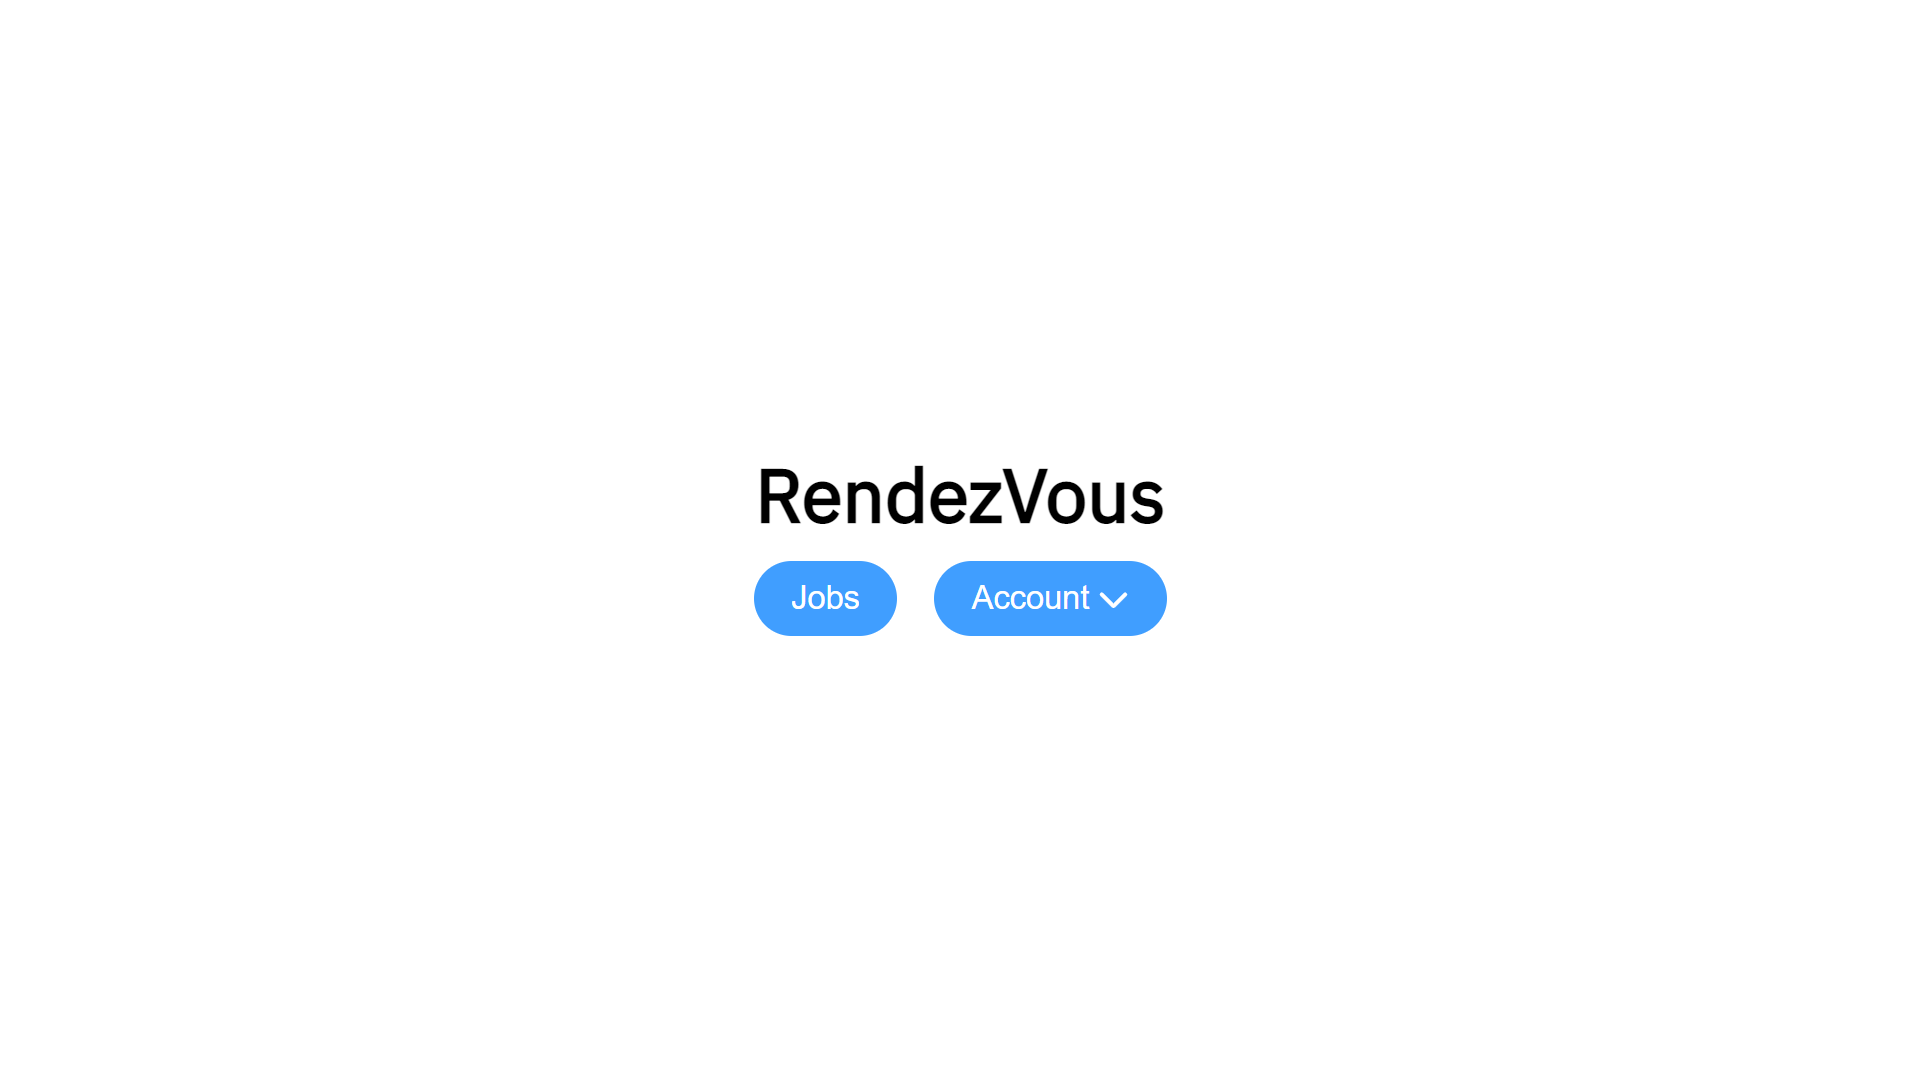
\includegraphics[width=0.9\linewidth]{06
        implementation/assets/auth flow/home page with auth.png}}
    \caption{Home page after authenticating}
  \end{subfigure}
  \begin{subfigure}{\subfigwidth}
    \centering
    \frame{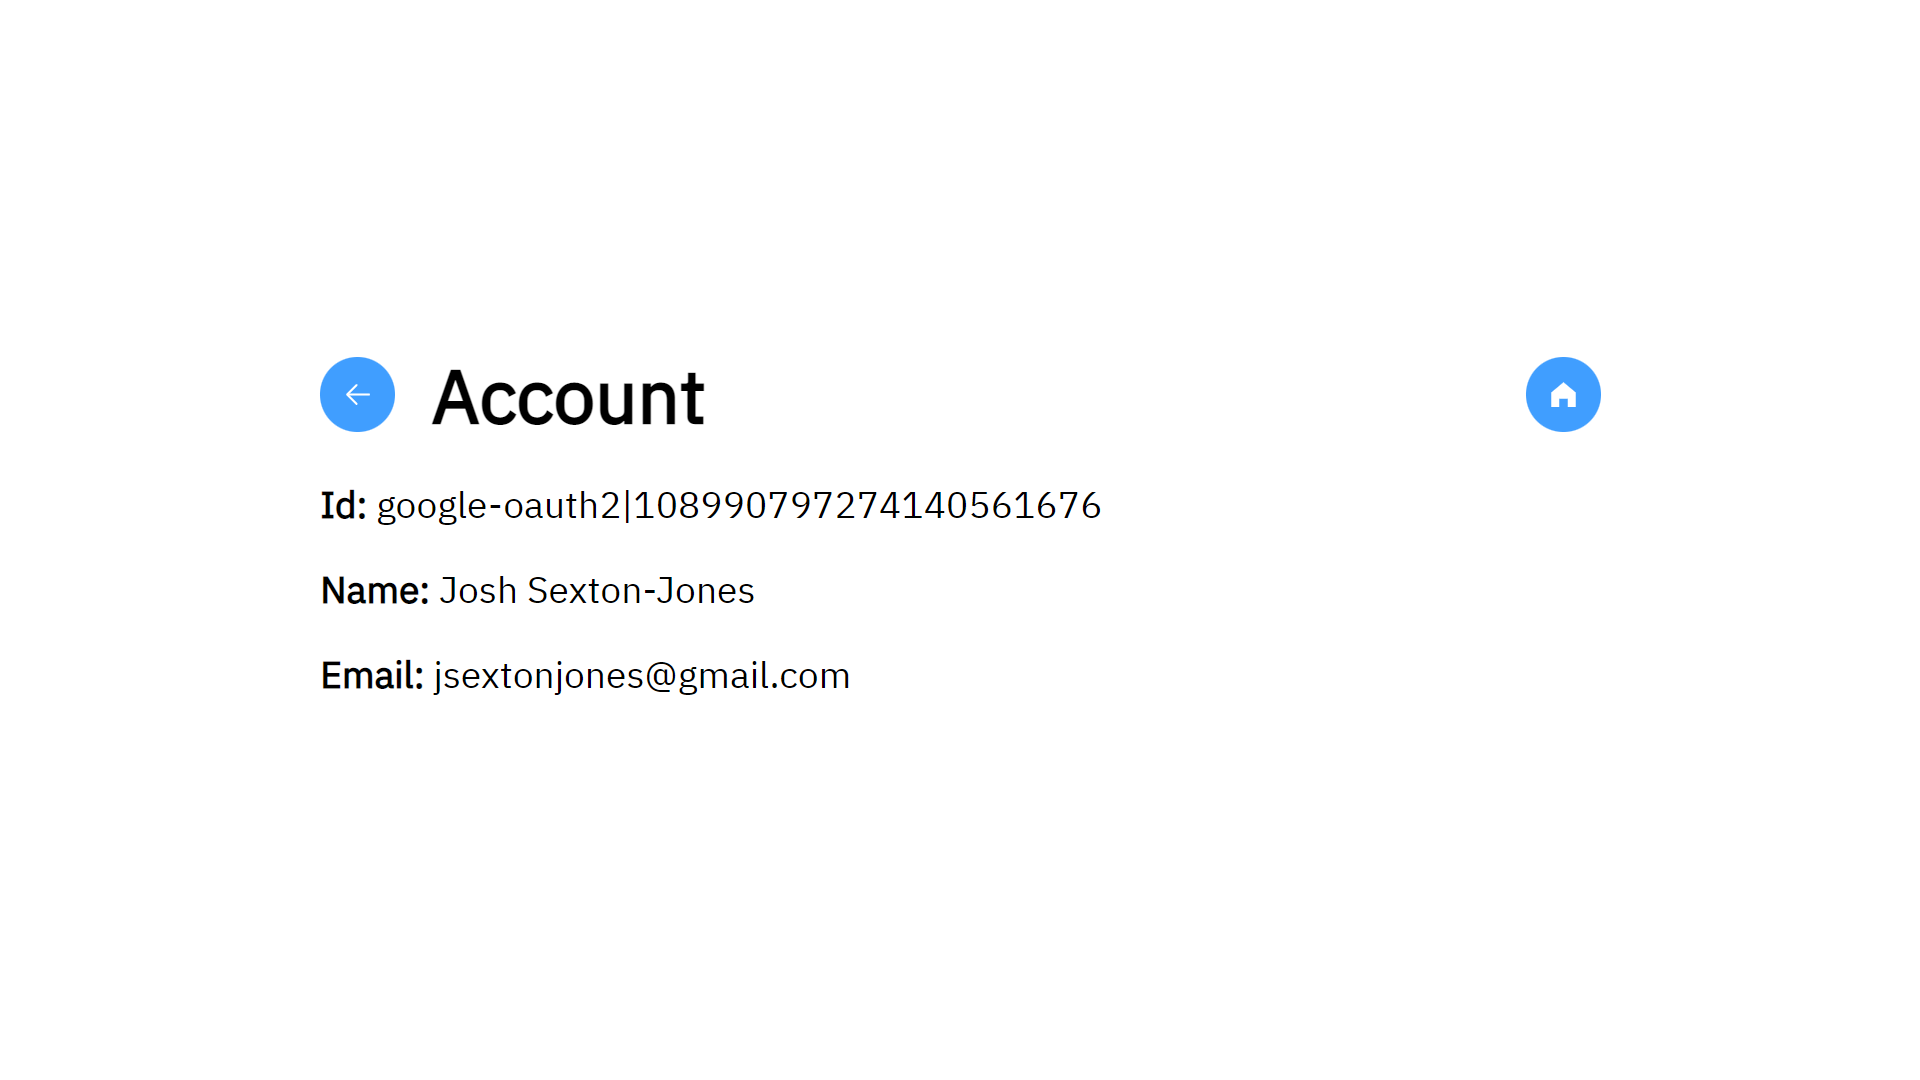
\includegraphics[width=0.9\linewidth]{06
        implementation/assets/auth flow/account page.png}}
    \caption{Account page}
  \end{subfigure}

  \caption{Frontend Authentication Flow}
  \label{fig:authFlow}
\end{figure}

In the backend, the access token sent from the frontend is
verified using the \gls{jwks} exposed by Auth0; once its
signature is verified, requests can proceed. 

\subsection{Accessing User Information}
